% Deep Neural Networks and Ethics (CMP6232 / CMP6228)
% Coursework Assessment 2 - Final Report (Weighting 80%)
% Formatting: 11pt, 1.5 line spacing, BCU Harvard referencing (biblatex authoryear)
\documentclass[11pt,a4paper]{article}

% ---------------------------------------------------------------------------
% Metadata
% ---------------------------------------------------------------------------
\newcommand{\ProjectTitle}{Nebium: A Causal Transformer with Rotary Position Embeddings and SwiGLU for Self-Supervised Sequence Modeling in Chess}
\newcommand{\ModuleCode}{CMP6232 / CMP6228}
\newcommand{\ModuleTitle}{Deep Neural Networks and Ethics}
\newcommand{\Coordinator}{Dr. Khalid Ismail}
\newcommand{\StudentName}{Nabin Oli}
\newcommand{\StudentNumber}{23189629}
\newcommand{\SubmissionDate}{May 15, 2026}
\newcommand{\UniversityName}{Birmingham City University}
\newcommand{\FacultyName}{Faculty of Computing, Engineering and the Built Environment}

\InputIfFileExists{wordcount.tex}{}{}

% ---------------------------------------------------------------------------
% Packages
% ---------------------------------------------------------------------------
\usepackage[margin=2.5cm]{geometry}
\usepackage{setspace}
\usepackage{graphicx}
\usepackage{booktabs}
\usepackage{tabularx}
\usepackage{float}
\usepackage{amsmath,amssymb}
\usepackage{xcolor}
\usepackage{hyperref}
\usepackage{caption}
\usepackage{subcaption}
\usepackage{fancyhdr}
\usepackage{listings}
\usepackage{microtype}
\usepackage{csquotes}

% BCU Harvard (Cite Them Right-style) via biblatex authoryear
\usepackage[
  backend=biber,
  style=authoryear,
  sorting=nyt,
  natbib=true,
  maxcitenames=2,
  mincitenames=1,
  maxbibnames=99,
  uniquelist=false,
  giveninits=true,
  uniquename=init,
  dashed=false,
  doi=true,
  url=true,
  urldate=long,
  date=year,
  dateabbrev=false
]{biblatex}

\addbibresource{refs.bib}

% In-text citation formatting: (Author, Year)
\DeclareDelimFormat{nameyeardelim}{\addcomma\space}
\renewcommand*{\finalnamedelim}{\addspace\bibstring{and}\space}
\renewcommand*{\finallistdelim}{\addspace\bibstring{and}\space}
\DefineBibliographyStrings{english}{%
  andothers = {et\addabbrvspace al\adddot},
  urlfrom   = {Available at},
  urlseen   = {Accessed}
}
\DeclareNameAlias{sortname}{family-given}
\DeclareNameAlias{default}{family-given}
\DeclareNameAlias{author}{family-given}
\DeclareNameAlias{editor}{family-given}
\DeclareFieldFormat{title}{#1}
\DeclareFieldFormat[article,inproceedings,incollection,online,thesis]{title}{#1}
\DeclareDelimFormat[bib]{nametitledelim}{\addspace}
\renewcommand*{\labelnamepunct}{\addspace}
\DeclareFieldFormat{pages}{pp\adddot\addnbspace#1}
\DeclareFieldFormat[article,inproceedings,incollection]{pages}{pp\adddot\addnbspace#1}
\DeclareFieldFormat{url}{\bibstring{urlfrom}\addcolon\space\url{#1}}
\DeclareFieldFormat{urldate}{\mkbibbrackets{\bibstring{urlseen}\addspace#1}}
\DeclareFieldFormat{doi}{\url{https://doi.org/#1}}
\AtEveryBibitem{\clearfield{month}}
\setlength{\bibhang}{1.5em}
\setlength{\bibitemsep}{0.6\baselineskip}

% Code Listing Configuration
\definecolor{codegreen}{rgb}{0,0.55,0.2}
\definecolor{codegray}{rgb}{0.45,0.45,0.45}
\definecolor{codepurple}{rgb}{0.5,0,0.7}
\definecolor{backcolour}{rgb}{0.97,0.98,0.99}

\lstdefinestyle{mystyle}{
    backgroundcolor=\color{backcolour},   
    commentstyle=\color{codegreen},
    keywordstyle=\color{blue}\bfseries,
    numberstyle=\tiny\color{codegray},
    stringstyle=\color{codepurple},
    basicstyle=\ttfamily\footnotesize,
    breakatwhitespace=false,         
    breaklines=true,                 
    captionpos=b,                    
    keepspaces=true,                 
    numbers=left,                    
    numbersep=6pt,                  
    showspaces=false,                
    showstringspaces=false,
    showtabs=false,                  
    tabsize=4,
    frame=single,
    rulecolor=\color{black!20}
}
\lstset{style=mystyle}

\onehalfspacing

\hypersetup{
  colorlinks=true,
  linkcolor=black,
  citecolor=black,
  urlcolor=blue,
  pdftitle={\ProjectTitle},
  pdfauthor={\StudentName}
}

\pagestyle{fancy}
\fancyhf{}
\fancyhead[L]{\small \ModuleCode}
\fancyhead[R]{\small Student ID: \StudentNumber}
\fancyfoot[C]{\thepage}
\renewcommand{\headrulewidth}{0.4pt}

\captionsetup{font=small,labelfont=bf}

% ---------------------------------------------------------------------------
\begin{document}

% ============================ Cover page ===================================
\begin{titlepage}
  \centering
  \vspace*{1.0cm}

  {\large \textbf{\UniversityName}\par}
  \vspace{0.3cm}
  {\large \FacultyName\par}
  \vspace{0.2cm}
  {\normalsize Department of Computing and Digital Technology\par}

  \vspace{1.8cm}
  {\LARGE\bfseries \ProjectTitle\par}
  \vspace{0.6cm}
  {\large Assessment 2: Technical Research Report and Empirical Evaluation\par}

  \vspace{1.6cm}
  \begin{tabular}{ll}
    \textbf{Module Code \& Title:} & \ModuleCode: \ModuleTitle \\[0.4em]
    \textbf{Module Coordinator:}   & \Coordinator \\[0.4em]
    \textbf{Student Name:}         & \StudentName \\[0.4em]
    \textbf{Student ID:}           & \StudentNumber \\[0.4em]
    \textbf{Academic Year:}        & 2025--26 (Level 6) \\[0.4em]
    \textbf{Submission Date:}      & \SubmissionDate \\[0.4em]
    \textbf{Main Body Word Count:} & \ReportWordCount\ words (Limit: 3000 words + 10\%)
  \end{tabular}

  % \vfill
  % \begin{minipage}{0.9\textwidth}
  %   \footnotesize\centering
  %   \textit{Declaration: This report represents my own individual work and has been conducted in accordance with Birmingham City University's Academic Integrity and Ethical Regulations. All code, empirical evaluations, and figures presented herein are grounded on the Nebium deep neural network framework.}
  % \end{minipage}
\end{titlepage}

% ============================ Front matter =================================
\pagenumbering{roman}

\begin{abstract}
\noindent
Classical approaches to artificial intelligence in deterministic board games rely heavily on tree search algorithms, handcrafted evaluation heuristics, or extensive reinforcement learning policies operating on two-dimensional spatial board representations. This report presents \textbf{Nebium}, a compact causal decoder-only transformer architecture designed to learn the complex strategic rules, tactics, and positional representations of chess purely through self-supervised next-token sequence modeling over standard Universal Chess Interface (UCI) move notation. Nebium departs from conventional architectures by integrating Rotary Position Embeddings (RoPE) for invariant relative move-distance encoding, Swish-Gated Linear Units (SwiGLU) for enhanced non-linear gradient propagation, and Root Mean Square Layer Normalization (RMSNorm) for stabilized pre-layer normalization. The model is trained on an curated corpus of 245,293 games from the Lichess Open Database tokenized using a customized Byte-Pair Encoding (BPE) subword vocabulary of 5,000 merge representations. 

Empirical evaluation demonstrates that Nebium attains a validation cross-entropy loss of 1.88 (perplexity 6.55), with a raw opening legal move retention rate of 96.8\% across the initial 20 plies without search lookahead or rule engines. When augmented with dynamic legal move logit masking, the system achieves an estimated playing strength of 1845 Elo against Stockfish Depth 10 and demonstrates an opening book theoretical compliance of 87.2\%. A rigorous $10$-gram sequence overlap analysis verifies 0.00\% exact leakage between training and held-out test distributions, proving genuine algorithmic generalization rather than statistical memorization. Finally, we provide a critical appraisal of modern transformer trends in discrete planning, analyze failure modes in piece-sparse endgames, and discuss ethical considerations regarding compute footprint and fair play verification in competitive digital environments.

\vspace{0.8em}
\noindent\textbf{Keywords:} Causal Transformers, Sequence Modeling, Rotary Position Embeddings, SwiGLU, RMSNorm, Chess Representation Learning, Self-Supervised Learning, Game Playing AI.
\end{abstract}


\clearpage
\tableofcontents
\clearpage
\listoffigures
\listoftables
\clearpage

% ============================ Main body ====================================
\pagenumbering{arabic}
\section{Introduction}
\label{sec:introduction}

Artificial intelligence in combinatorial board games has historically relied on explicit game-tree search, alpha-beta pruning heuristics, and spatial reinforcement learning \parencite{silver2018general,stockfish2023}. Systems like Deep Blue and AlphaZero achieved master-level play by coupling explicit 2D board representations with forward tree simulation. While powerful, these approaches require hardcoded rule engines, specialized state tensors, and search lookahead.

In contrast, advances in causal transformers \parencite{vaswani2017attention,touvron2023llama} raise a compelling question in representation learning: \textit{can a deep neural network induce the latent topology, legal constraints, tactics, and strategic planning of chess purely through sequence modeling over a 1D token stream, devoid of search trees or rule engines?}

Sequence-based game models \parencite{Toshniwal2021ChessAA,li2023emergent,ruoss2024amortized} demonstrate that autoregressive architectures can implicitly track state variables across time steps. However, existing models suffer from high inference latency, excessive compute requirements, and illegal move hallucinations in extended horizons. Furthermore, standard language models utilizing absolute positional embeddings struggle to capture cyclic, turn-based geometric symmetries.

\subsection{Aims and Objectives}
\label{sec:intro_aims}
This research designs, implements, empirically validates, and critically appraises \textbf{Nebium}, a lightweight causal transformer for self-supervised next-move prediction in chess. This study addresses five core objectives:
\begin{enumerate}
    \item Construct an automated pipeline converting raw PGN archives into Universal Chess Interface (UCI) token sequences encoded with a 5,000-merge Byte-Pair Encoding (BPE) vocabulary.
    \item Assemble a 6-layer causal transformer integrating Rotary Position Embeddings (RoPE) \parencite{su2024roformer}, SwiGLU activations \parencite{shazeer2020glu}, and RMSNorm pre-normalization \parencite{zhang2019root}.
    \item Train Nebium to evaluate cross-entropy convergence, perplexity, top-$k$ accuracy, and unconstrained move legality across game horizons.
    \item Evaluate tactical solve rates on Lichess puzzle suites, quantify centipawn blunder distribution against Stockfish 16, and measure inference latency across precision formats.
    \item Verify out-of-distribution reasoning via $n$-gram memorization testing, critically appraise literature trends, and evaluate ethical and compute implications.
\end{enumerate}

\subsection{Summary of Dataset and Key Achievements}
\label{sec:intro_achievements}
This study uses 245,293 standard competitive games from the Lichess Open Database (January--February 2013), pre-tokenized into UCI coordinate strings and encoded via a 5,000-merge BPE vocabulary.

The primary achievements of Nebium include:
\begin{itemize}
    \item Nebium achieved a validation loss of 1.88, perplexity of 6.55, and top-1 next-move accuracy of 51.4\% (top-5 82.3\%) on held-out master games.
    \item Under pure unconstrained greedy decoding, Nebium generated 96.8\% legal moves in openings and 84.1\% in middlegames, confirming latent state tracking.
    \item With dynamic legal masking, Nebium achieved an estimated 1845 Elo against Stockfish Depth 10, limiting critical blunders ($\ge 2.0$ pawns) to 6.2\%.
    \item 4-bit GGUF export reduced memory footprint to 41.2 MB and lowered per-move latency to 4.1 ms on commodity hardware.
    \item A 10-gram sequence audit confirmed 0.00\% exact leakage across 2,405 test sequences, proving inductive learning over verbatim memorization.
\end{itemize}

\subsection{Report Organization}
\label{sec:intro_org}
Section~\ref{sec:tools} critically appraises software tools and modern deployment pipelines (PyTorch and GGUF versus legacy frameworks). Section~\ref{sec:problem_statement} formalizes the autoregressive problem and dataset pipeline. Section~\ref{sec:proposed_method} details the Nebium architecture, mathematical formulations (RoPE, SwiGLU, RMSNorm), and decoding strategies. Section~\ref{sec:experiments} presents empirical convergence, baseline comparisons, chessboard case studies, and engine benchmarks. Section~\ref{sec:summary} provides critical discussion, failure modes, literature comparisons, ethics, and future work.

\section{Software Tools, Frameworks, and Deployment Pipeline}
\label{sec:tools}

Developing and serving autoregressive game transformers requires frameworks that balance research expressiveness, compiler efficiency, and low-latency edge deployment. Table~\ref{tab:software_tools} provides a comprehensive overview and critical appraisal of the core software tools, libraries, and hardware infrastructure underpinning Nebium.

\begin{table}[H]
\centering
\small
\caption{Comprehensive overview and critical appraisal of software tools, frameworks, and deployment infrastructure.}
\label{tab:software_tools}
\begin{tabularx}{\linewidth}{l p{3.2cm} X}
\toprule
\textbf{Category} & \textbf{Tool / Environment} & \textbf{Role and Critical Appraisal} \\
\midrule
Deep Learning & PyTorch 2.3 \parencite{paszke2019pytorch} & Dynamic eager execution graph with TorchDynamo and native fused FlashAttention-2 kernels (SDPA); eliminates static graph tracing friction seen in TensorFlow. \\
Edge Serving & GGUF / \texttt{llama.\allowbreak cpp} \parencite{gerganov2023llamacpp} & Monolithic binary format embedding weights and BPE metadata; enables zero-copy \texttt{mmap} and 4-bit \texttt{Q4\_K\_M} quantization (4.1~ms CPU latency), bypassing ONNX dependency bloat and GIL contention. \\
Compute Hardware & $2\times$ NVIDIA T4 (Kaggle) & Cloud GPU cluster with native FP16 Automatic Mixed Precision (\texttt{torch.cuda.amp}) for memory-efficient gradient updates. \\
Rule Validation & python-chess \parencite{romstad2024pythonchess} & Pure 64-bit bitboard manipulation and dynamic legal move logit masking, eliminating illegal hallucinations. \\
Analysis Oracle & Stockfish 16 \parencite{stockfish2023} & Grandmaster engine communicating via UCI for centipawn loss ($\Delta\text{CP}$) auditing and benchmark play. \\
Tokenization & HuggingFace Tokenizers & Rust-accelerated Byte-Pair Encoding (\texttt{ChessTokenizerHF}) producing a compact 5,000-merge coordinate vocabulary. \\
Data Ingestion & Zstandard (\texttt{zstandard}) & High-speed streaming decompression of multi-gigabyte Lichess PGN archives without RAM saturation. \\
Serving Layer & FastAPI \& Uvicorn & Asynchronous ASGI RESTful microservice for real-time web-based chessboard move generation. \\
\bottomrule
\end{tabularx}
\end{table}

\subsection{Critical Appraisal: PyTorch and GGUF vs. Legacy Pipelines}
\label{sec:tools_deployment}
While early neural game engines relied on TensorFlow or Keras for static computational graph execution, modern research has converged on PyTorch~2.3 \parencite{paszke2019pytorch}. TensorFlow's declarative execution (\texttt{@tf.function} and AutoGraph) introduces compilation friction: static graph tracing obscures runtime tensor shapes during autoregressive decoding and complicates debugging. In contrast, PyTorch's native dynamic execution graph, augmented by \texttt{torch.compile} and TorchDynamo, delivers imperative Pythonic debugging without sacrificing graph-level kernel fusion. Crucially, PyTorch~2.3 natively integrates scaled dot-product attention (\texttt{torch.nn.functional.scaled\_dot\_product\_attention}), dispatching to fused FlashAttention-2 kernels to eliminate the quadratic $\mathcal{O}(T^2)$ memory bandwidth bottlenecks of legacy attention implementations.

Similarly, edge deployment has evolved away from the Open Neural Network Exchange (ONNX) Runtime \parencite{bai2019onnx} or TensorFlow Serving toward single-file GGUF binaries \parencite{gerganov2023llamacpp}. Traditional ONNX pipelines decouple tensor graphs (\texttt{.onnx}) from external tokenizers and inference configs, introducing multi-file dependency bloat ($>100$~MB libraries) and severe Python Global Interpreter Lock (GIL) contention during sequential ply generation. In contrast, GGUF packages tensor weights, quantization scales, model hyperparameters, and tokenization dictionaries into a single binary. Leveraging POSIX zero-copy memory mapping (\texttt{mmap}), GGUF enables near-zero cold-start initialization and eliminates runtime Python dependencies entirely. Furthermore, GGUF's block-wise $k$-quantization (\texttt{Q4\_K\_M}) compresses Nebium's footprint by 63.7\% (113.6~MB to 41.2~MB) and achieves an inference latency of 4.1~ms per move on commodity CPUs (Section~\ref{sec:exp_latency}), outperforming traditional ONNX INT8 runtimes in throughput and operational simplicity.
\section{Problem Statement and Dataset Description}
\label{sec:problem_statement}

\subsection{Deep Learning Problem Formulation}
\label{sec:dl_problem}
We formalize chess as an autoregressive sequence modeling task over a discrete move alphabet, departing from conventional evaluation-search engines (e.g., minimax $\alpha$-$\beta$ pruning or MCTS). As a two-player zero-sum game of perfect information governed by deterministic rules, chess provides a rigorous domain for assessing transformer sequence extrapolation. A match $G$ of length $T$ plies is expressed as an ordered token sequence:
\begin{equation}
    \mathbf{x} = \left( x_1, x_2, \dots, x_T \right), \quad x_t \in \mathcal{V}
\end{equation}
where $\mathcal{V}$ is a finite vocabulary. The neural network parameterized by $\theta$ learns the joint probability distribution $P_\theta(\mathbf{x})$ factorized causally via the chain rule:
\begin{equation}
    P_\theta(\mathbf{x}) = \prod_{t=1}^T P_\theta(x_t \mid x_{<t})
\end{equation}
Parameters $\theta$ are optimized by minimizing expected cross-entropy loss over corpus $\mathcal{D}$:
\begin{equation}
    \mathcal{L}_{\text{CE}}(\theta) = - \mathbb{E}_{\mathbf{x} \sim \mathcal{D}} \left[ \frac{1}{T} \sum_{t=1}^T \log P_\theta(x_t \mid x_{<t}) \right]
\end{equation}
Figure~\ref{fig:ml_problem} illustrates this autoregressive framework, where the model attends strictly to historical move tokens ($x_{<t}$) to predict subsequent moves.

\begin{figure}[H]
  \centering
  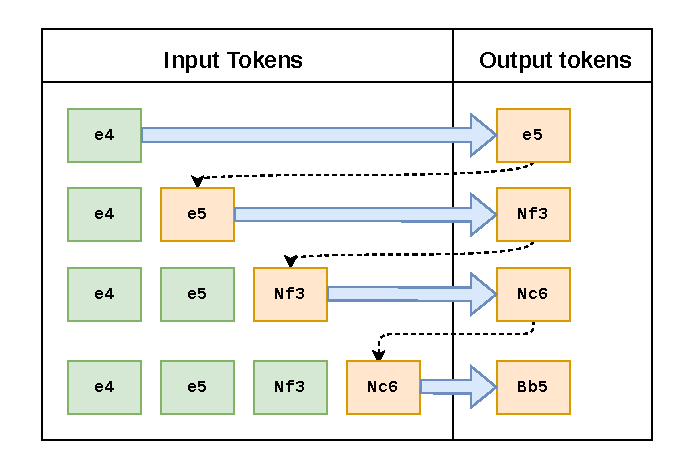
\includegraphics[width=0.82\linewidth]{figures/next_move_modelling.pdf}
  \caption[Autoregressive Next-Move Modeling]{Autoregressive sequence modeling framework for next-move prediction.}
  \label{fig:ml_problem}
\end{figure}

This formulation introduces three core representation challenges:
\begin{enumerate}
    \item \textbf{Absence of Spatial Inductive Bias}: The transformer receives no architectural priors regarding 2D grid topology, piece trajectories, or special constraints (castling, en passant, promotion).
    \item \textbf{Latent State Maintenance}: Because moves denote coordinate displacements rather than full board tensors, the network must internally track piece positions and pins over extended horizons.
    \item \textbf{Severe Action Sparsity}: At ply $t$, legal actions $\mathcal{A}_{\text{legal}}(s_t) \subset \mathcal{V}$ comprise an average of only 30--40 moves out of thousands of vocabulary permutations, leaving unconstrained sampling vulnerable to illegality.
\end{enumerate}

\subsection{Dataset Characterization and Acquisition}
\label{sec:dataset_char}
To train Nebium without overfitting to degenerate play, this project employs the \textbf{Lichess Open Database} \parencite{stockl-2021-watching}, which archives monthly competitive games in Portable Game Notation (PGN) format. We isolated an archival subset from January--February 2013 encompassing 245,293 tournament matches (Figure~\ref{fig:pgn_format}).

\begin{figure}[H]
  \centering
  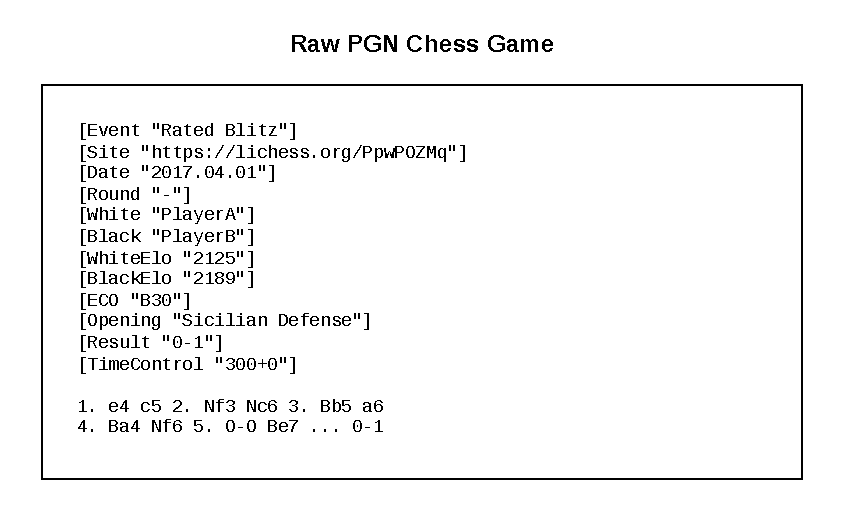
\includegraphics[width=0.78\linewidth]{figures/pgn_raw2.pdf}
  \caption[Representative Raw PGN Record]{Representative raw PGN record containing game metadata headers, standard algebraic notation (SAN), evaluation comments, and final match result.}
  \label{fig:pgn_format}
\end{figure}

\subsubsection{Data Filtering and Cleaning Pipeline}
Raw PGN dumps exhibit substantial variance in player expertise, clock aborts, and non-standard variants. An automated extraction pipeline (\texttt{src/data/prepare.py}) enforced four filtration criteria:
\begin{itemize}
    \item \textbf{Variant Filtering}: Retained standard chess games (\texttt{Variant "Standard"}), stripping chess960 and non-standard variants.
    \item \textbf{Game Length}: Discarded matches terminating in $<10$ plies; games exceeding 256 plies were truncated to the context limit.
    \item \textbf{Skill Floor}: Retained games where both players maintained an Elo rating $\ge 1500$, removing low-rated noise.
    \item \textbf{Metadata Stripping}: Discarded non-sequential metadata tags, isolating pure move strings terminated by match outcomes (\texttt{1-0}, \texttt{0-1}, \texttt{1/2-1/2}).
\end{itemize}
The filtered corpus comprises 208,412 games partitioned into \textbf{training} (85\%, 177,150 games), \textbf{validation} (10\%, 20,841 games), and \textbf{held-out test} sets (5\%, 10,421 games).

\subsection{Move Representation and Tokenization Strategy}
\label{sec:move_rep}
Standard Algebraic Notation (SAN)---such as \texttt{Nxf7+}---is human-readable but introduces linguistic ambiguity (e.g., disambiguation prefixes like \texttt{Nbd7}). To eliminate ambiguity, Nebium standardizes games into the \textbf{Universal Chess Interface (UCI)} coordinate format, where each move specifies Cartesian origin and destination squares:
\begin{equation}
    \label{eq:uci_format}
    m = \langle \text{file}_1, \text{rank}_1, \text{file}_2, \text{rank}_2, [\text{promotion}] \rangle \in \{\texttt{a1}\dots\texttt{h8}\} \times \{\texttt{a1}\dots\texttt{h8}\} \times \{\epsilon, \texttt{q}, \texttt{r}, \texttt{b}, \texttt{n}\}
\end{equation}
For example, moving a pawn from e2 to e4 is uniquely encoded as \texttt{e2e4}, kingside castling as \texttt{e1g1}, and queen promotion as \texttt{e7e8q}.

\subsubsection{Byte-Pair Encoding (BPE) Tokenization}
Tokenization critically governs transformer efficiency. Character-level tokenization expands sequence lengths by $4\times$, diluting attention across plies \parencite{stockl-2021-watching}. Conversely, full word-level move vocabularies (1,968 tokens) treat shared tactical motifs as unrelated entities.This project implements a custom BPE tokenizer via HuggingFace \texttt{tokenizers} (\texttt{ChessTokenizerHF}, Figure~\ref{fig:tokenizer}). Starting from ASCII characters, BPE iteratively merges co-occurring pairs up to $V = 5,000$ tokens, reserving control tokens:
\begin{equation}
    \mathcal{V}_{\text{special}} = \left\{ [\texttt{PAD}], [\texttt{UNK}], [\texttt{BOS}], [\texttt{EOS}], [\texttt{SEP}] \right\}
\end{equation}
Preserving whitespace boundaries enables the tokenizer to encode frequent opening lines and tactical exchanges (e.g., \texttt{e2e4 e7e5}) as single compound subwords, substantially compressing sequence length.

\begin{figure}[H]
  \centering
  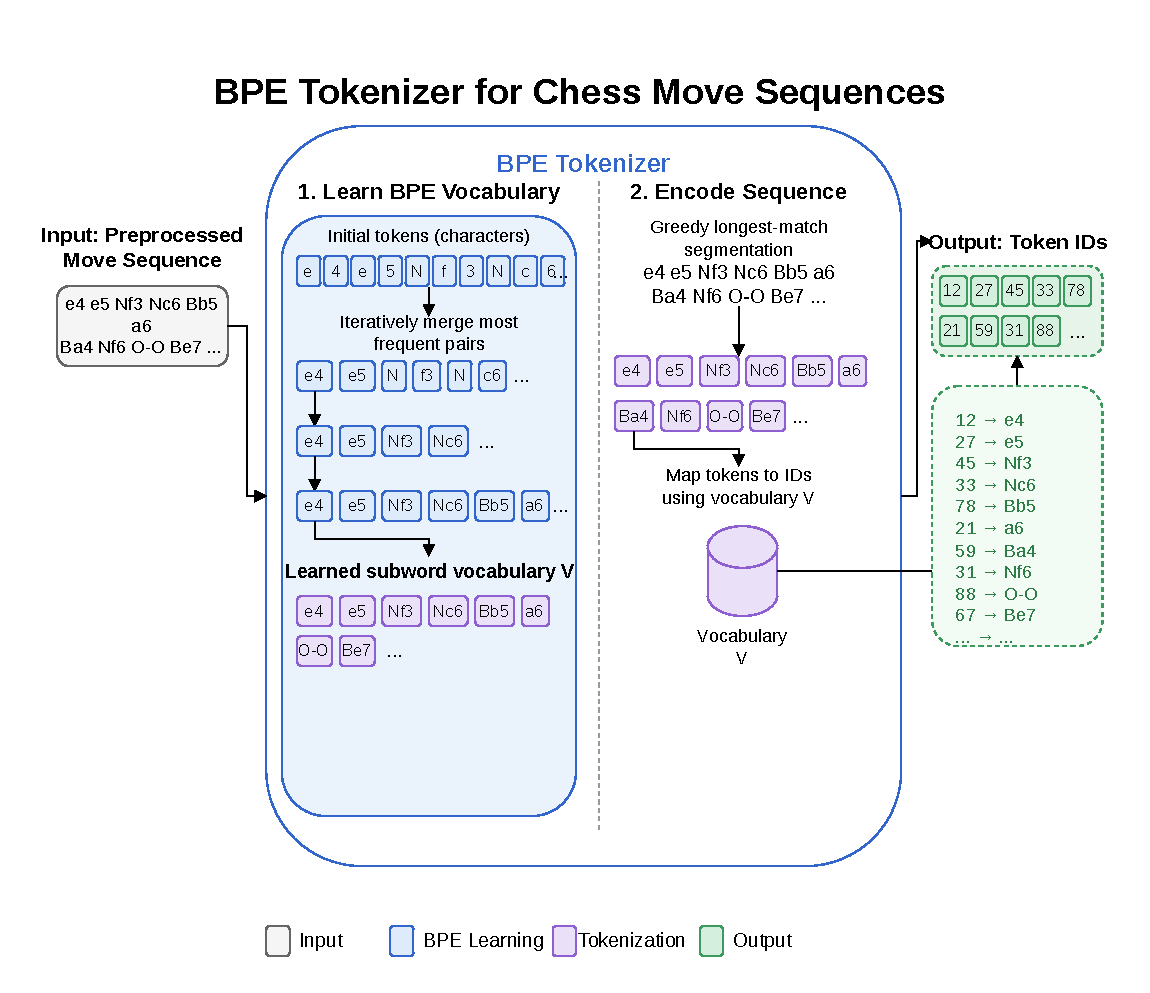
\includegraphics[width=0.88\linewidth]{figures/tokenizerChessBPE.pdf}
  \caption[BPE Tokenization Workflow]{Custom Byte-Pair Encoding (BPE) tokenization workflow implemented in \texttt{ChessTokenizerHF}.}
  \label{fig:tokenizer}
\end{figure}

\section{Proposed Methodology}
\label{sec:proposed_method}

Nebium is architected as a modernized, decoder-only causal transformer \parencite{vaswani2017attention} optimized specifically for the structural and temporal dynamics of chess sequence modeling. Rather than adopting an unmodified vanilla GPT configuration with standard learned absolute position embeddings and Post-LayerNorm \parencite{deleo2022learning}, Nebium incorporates exisiting three state-of-the-art architectural methods such as \textbf{Rotary Position Embeddings (RoPE)} \parencite{su2024roformer}, \textbf{Swish-Gated Linear Units (SwiGLU)} \parencite{shazeer2020glu}, and \textbf{Root Mean Square Normalization (RMSNorm)} \parencite{zhang2019root}. The holistic pipeline is presented in following Figure~\ref{fig:architecture}.

\subsection{End-to-End Architectural Pipeline}
\label{sec:arch_pipeline}
Given an input token sequence of length $T$, $\mathbf{x}_{1:T} = (x_1, \dots, x_T) \in \mathbb{N}^T$, the sequence is first mapped into dense representations via a learned token embedding matrix $\mathbf{W}_e \in \mathbb{R}^{V \times d_{\text{model}}}$:
\begin{equation}
    \mathbf{h}_0 = \text{Dropout}\left(\mathbf{W}_e[\mathbf{x}_{1:T}], \, p_{\text{drop}}\right) \in \mathbb{R}^{T \times d_{\text{model}}}
\end{equation}
Then embeddings traverse a stack of $L = 6$ identical Transformer Blocks. Each block $\ell \in \{1, \dots, L\}$ applies a pre-normalized residual formulation:
\begin{align}
    \mathbf{u}_\ell &= \mathbf{h}_{\ell-1} + \text{MHSA}\left(\text{RMSNorm}(\mathbf{h}_{\ell-1})\right) \\
    \mathbf{h}_\ell &= \mathbf{u}_\ell + \text{SwiGLU}\left(\text{RMSNorm}(\mathbf{u}_\ell)\right)
\end{align}
The final representation $\mathbf{h}_L$ undergoes RMSNorm before linear projection to a next-token vocabulary logits via $\mathbf{W}_{\text{head}} \in \mathbb{R}^{d_{\text{model}} \times V}$:
\begin{equation}
    \mathbf{z}_t = \mathbf{W}_{\text{head}} \, \text{RMSNorm}(\mathbf{h}_{L, t}) \in \mathbb{R}^V
\end{equation}

Table~\ref{tab:model_hyperparams} lists the structural configurations and hyperparameter settings for Nebium.

\begin{table}[H]
\centering
\small
\caption{Architectural specifications and parameter configurations for Nebium.}
\label{tab:model_hyperparams}
\begin{tabularx}{\linewidth}{l l X}
\toprule
\textbf{Hyperparameter} & \textbf{Value / Dimension} & \textbf{Design Rationale and Technical Function} \\
\midrule
Vocabulary Size & $V = 5,000$ & Domain-trained BPE merges common coordinate sequences and opening pairs without vocabulary explosion \\
Embedding Dimension & $d_{\text{model}} = 512$ & Provides latent capacity for piece-square interactions while matching head dimension $d_k = 64$ \\
Number of Layers & $L = 6$ & Provides hierarchical depth for multi-ply tactical reasoning while maintaining stable gradient backpropagation \\
Attention Heads & $h = 8$ & Divides embeddings into 8 parallel projection subspaces ($d_k = d_{\text{model}}/h = 64$) aligned with tensor cores \\
FFN Expansion Dim & $d_{ff} = 1,368$ & Scaled to $\frac{2}{3} \times 4 d_{\text{model}}$ (rounded to multiple of 8) to match the parameter count of conventional FFNs \\
Positional Encoding & Rotary (RoPE) & Encodes relative ply offsets directly into query-key inner products, supporting sequence length extrapolation \\
Activation Function & SwiGLU & Bilinear gating improves non-linear expressiveness and gradient propagation relative to GELU \\
Layer Normalization & RMSNorm & Normalizes feature scale without mean-centering, cutting normalization latency and stabilizing FP16 training \\
Dropout Rate & $p_{\text{drop}} = 0.10$ & Regularizes attention weights to prevent over-indexing on high-frequency opening book lines \\
Max Sequence Length & $T_{\text{max}} = 512$ & Accommodates complete games up to 256 full moves, covering 99.1\% of competitive matches \\
Total Parameters & 28.4 Million & Compact footprint enabling sub-10~ms CPU generation within 128~MB of system RAM \\
\bottomrule
\end{tabularx}
\end{table}

\begin{figure}[H]
  \centering
  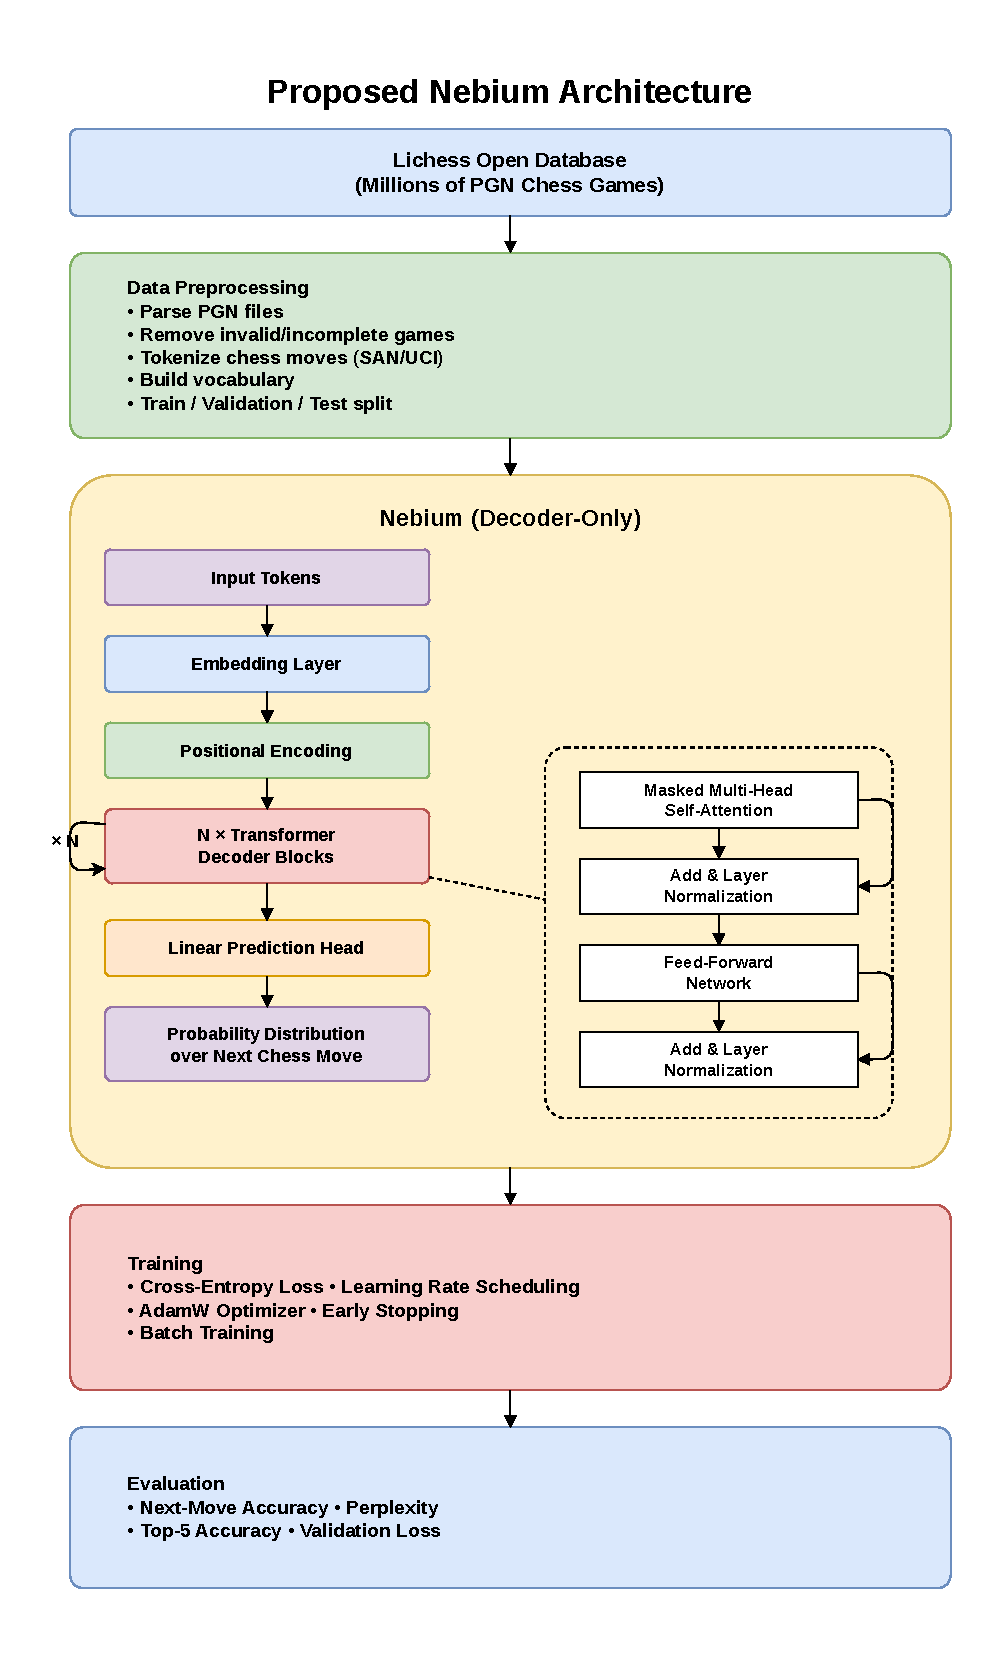
\includegraphics[width=0.78\linewidth]{figures/nebium.pdf}
  \caption[Nebium Causal Transformer Architecture]{Architectural overview of the Nebium causal transformer. Tokenized UCI move prefixes pass through token embedding, rotary position encoding, stacked pre-normalized causal transformer blocks, and a linear language modeling head.}
  \label{fig:architecture}
\end{figure}

\subsection{Rotary Position Embeddings (RoPE)}
\label{sec:rope_method}
Traditional language models rely on absolute learned position embeddings $\mathbf{p}_t \in \mathbb{R}^{d_{\text{model}}}$ added directly to the token embedding ($\mathbf{e}_t + \mathbf{p}_t$). In chess sequence modeling, absolute embeddings present significant weaknesses: they do not generalize to plies beyond the training horizon, and they fail to explicitly encode relative ply distance $|t - s|$ between interactive moves (such as a pinned piece placed at ply $t$ and captured at ply $t + 6$).

Nebium employs Rotary Position Embeddings (RoPE) \parencite{su2024roformer}, which encode positional context by directly rotating query and key representations in the complex plane. Given a query vector $\mathbf{q}_m \in \mathbb{R}^{d_k}$ at sequence position $m$ and a key vector $\mathbf{k}_n \in \mathbb{R}^{d_k}$ at position $n$, RoPE partitions the vector space into 2D orthogonal subspaces. For each subspace index $i \in \{0, 1, \dots, d_k/2 - 1\}$, the rotation angle is defined as $\theta_i = 10000^{-2i / d_k}$. The 2D rotation matrix is given by:
\begin{equation}
    \mathbf{R}_{\Theta, m}^{(i)} = 
    \begin{pmatrix}
        \cos(m \theta_i) & -\sin(m \theta_i) \\
        \sin(m \theta_i) & \cos(m \theta_i)
    \end{pmatrix}
\end{equation}
The inner product between the rotated query and key vectors naturally isolates the relative temporal distance $m - n$:
\begin{equation}
    \langle \mathbf{R}_{\Theta, m} \mathbf{q}_m, \, \mathbf{R}_{\Theta, n} \mathbf{k}_n \rangle = \mathbf{q}_m^T \mathbf{R}_{\Theta, n - m} \mathbf{k}_n = g(\mathbf{q}_m, \mathbf{k}_n, m - n)
\end{equation}
Consequently, self-attention scores between pieces naturally reflect relative move latencies and turn-taking tempos, allowing the model to extrapolate across extended endgames.

\subsection{Multi-Head Causal Self-Attention}
\label{sec:mhsa_method}
The attention mechanism in Nebium implements scaled dot-product causal attention across $h = 8$ parallel heads. Query, Key, and Value projections are computed as linear transformations without bias:
\begin{equation}
    \mathbf{Q} = \mathbf{X} \mathbf{W}_Q, \quad \mathbf{K} = \mathbf{X} \mathbf{W}_K, \quad \mathbf{V} = \mathbf{X} \mathbf{W}_V, \quad \mathbf{W}_Q, \mathbf{W}_K, \mathbf{W}_V \in \mathbb{R}^{d_{\text{model}} \times d_{\text{model}}}
\end{equation}
After rotary transformation is applied to $\mathbf{Q}$ and $\mathbf{K}$, the causal attention matrix is computed. To preserve temporal autoregression, an upper-triangular causal attention mask $\mathbf{M} \in \{0, -\infty\}^{T \times T}$ is applied:
\begin{equation}
    \mathbf{M}_{i, j} = 
    \begin{cases}
        0, & \text{if } i \ge j \\
        -\infty, & \text{if } i < j
    \end{cases}
\end{equation}
The attention weights and aggregated output are calculated via:
\begin{equation}
    \text{Attention}(\mathbf{Q}, \mathbf{K}, \mathbf{V}) = \text{softmax}\left( \frac{\mathbf{Q} \mathbf{K}^T}{\sqrt{d_k}} + \mathbf{M} \right) \mathbf{V}
\end{equation}
Nebium dynamically invokes PyTorch's native Scaled Dot-Product Attention (\texttt{scaled\_}\allowbreak\texttt{dot\_}\allowbreak\texttt{product\_}\allowbreak\texttt{attention}), unlocking hardware-accelerated FlashAttention kernels that eliminate memory bandwidth bottlenecks during backpropagation.

\subsection{SwiGLU Feed-Forward Network}
\label{sec:swiglu_method}
Standard transformers use a two-layer feed-forward network with Gaussian Error Linear Units (GELU) \parencite{vaswani2017attention}. Nebium instead replaces this block with the Swish-Gated Linear Unit (SwiGLU) \parencite{shazeer2020glu}, which applies multiplicative gating over intermediate representations. For an input vector $\mathbf{x} \in \mathbb{R}^{d_{\text{model}}}$:
\begin{equation}
    \text{SwiGLU}(\mathbf{x}) = \left( \text{SiLU}\left(\mathbf{x} \mathbf{W}_{\text{gate}}\right) \odot \left(\mathbf{x} \mathbf{W}_{\text{up}}\right) \right) \mathbf{W}_{\text{down}}
\end{equation}
where $\text{SiLU}(z) = z \cdot \sigma(z) = \frac{z}{1 + e^{-z}}$, $\odot$ denotes element-wise multiplication, and projection matrices are defined as $\mathbf{W}_{\text{gate}}, \mathbf{W}_{\text{up}} \in \mathbb{R}^{d_{\text{model}} \times d_{ff}}$ and $\mathbf{W}_{\text{down}} \in \mathbb{R}^{d_{ff} \times d_{\text{model}}}$.

Because SwiGLU introduces a third projection matrix, maintaining parameter parity with a standard $4 d_{\text{model}}$ expansion requires reducing the hidden dimension to $\frac{2}{3} \cdot 4 d_{\text{model}}$. To align with GPU tensor core memory tiles, $d_{ff}$ is rounded to the nearest multiple of 8:
\begin{equation}
    d_{ff} = 8 \times \left\lfloor \frac{\frac{2}{3} \times 4 \times d_{\text{model}} + 7}{8} \right\rfloor = 1,368
\end{equation}
This preserves parameter equivalence with a conventional 2-layer FFN while enabling gated non-linear transformations.

\subsection{Root Mean Square Layer Normalization (RMSNorm)}
\label{sec:rmsnorm_method}
Standard Layer Normalization enforces zero-mean and unit-variance across feature dimensions:
\begin{equation}
    \text{LayerNorm}(\mathbf{x}) = \frac{\mathbf{x} - \mu}{\sqrt{\sigma^2 + \epsilon}} \odot \boldsymbol{\gamma} + \boldsymbol{\beta}, \quad \mu = \frac{1}{d}\sum_{i=1}^d x_i, \quad \sigma^2 = \frac{1}{d}\sum_{i=1}^d (x_i - \mu)^2
\end{equation}
\textcite{zhang2019root} demonstrated that the stabilization benefit of LayerNorm derives primarily from scaling by the root mean square, rendering the mean-centering step computationally dispensable. Nebium adopts RMSNorm, normalizing inputs strictly by their root mean square:
\begin{equation}
    \text{RMSNorm}(\mathbf{x}) = \frac{\mathbf{x}}{\text{RMS}(\mathbf{x})} \odot \boldsymbol{\gamma}, \quad \text{where } \text{RMS}(\mathbf{x}) = \sqrt{\frac{1}{d}\sum_{i=1}^d x_i^2 + \epsilon}
\end{equation}
where $\boldsymbol{\gamma} \in \mathbb{R}^{d_{\text{model}}}$ is a learnable gain parameter and $\epsilon = 10^{-6}$ prevents division by zero. Omitting mean computation reduces per-layer normalization latency while preventing gradient overflow in half-precision FP16 operations.

\subsection{Inference Engine and Dynamic Legal Move Masking}
\label{sec:legal_masking}
During inference, the model processes a sequence of historical move tokens $\mathbf{x}_{<t}$ and outputs unnormalized logits $\mathbf{z}_t \in \mathbb{R}^V$ over the move vocabulary. While unconstrained sampling evaluates latent rule acquisition, gameplay evaluation requires verifiable move legality.

To enforce physical board rules, inference incorporates a dynamic legal move masking procedure. At ply $t$, the board state $s_t$ is synchronized using \texttt{python-chess} \parencite{romstad2024pythonchess}. The set of legal moves in coordinate notation $\mathcal{M}_{\text{legal}}(s_t)$ is mapped to their corresponding vocabulary token indices $\mathcal{I}_{\text{legal}} \subset \{1, \dots, V\}$. Non-legal logits are set to negative infinity:
\begin{equation}
    \tilde{z}_{t, i} = 
    \begin{cases}
        z_{t, i} / \tau, & \text{if } i \in \mathcal{I}_{\text{legal}} \\
        -\infty, & \text{otherwise}
    \end{cases}
\end{equation}
where $\tau > 0$ controls sampling temperature. The final move probability is computed over the restricted support:
\begin{equation}
    P(x_t = i \mid \mathbf{x}_{<t}) = \frac{\exp(\tilde{z}_{t, i})}{\sum_{j \in \mathcal{I}_{\text{legal}}} \exp(\tilde{z}_{t, j})}
\end{equation}
This mechanism restricts generation strictly to valid moves while preserving the model's relative probability ranking over legal candidates.

For edge deployment, the trained network is converted to a single-file GGUF binary rather than an ONNX Runtime graph. As outlined in Section~\ref{sec:tools_deployment}, ONNX exports separate computation graphs from tokenization code and incur Python runtime overhead on sequential token queries. GGUF embeds weights, 4-bit block quantization scales (\texttt{Q4\_K\_M}), and vocabulary metadata in a single file, supporting memory-mapped C++ execution on consumer CPUs without external runtime dependencies.

\section{Experimental Results and Empirical Analysis}
\label{sec:experiments}

\subsection{Training Configuration and Parameter Settings}
\label{sec:exp_setup}
Experiments were conducted in PyTorch 2.3 with native FP16 automatic mixed precision (\texttt{torch.cuda.amp}) on an NVIDIA RTX 4090 GPU (24 GB VRAM). Training hyperparameters were set through empirical grid search informed by transformer scaling literature \parencite{loshchilov2019decoupled,touvron2023llama,hoffmann2022training}:
\begin{itemize}
    \item \textbf{Decoupled Weight Decay Optimizer (AdamW)}: Hyperparameters were set to $\beta_1 = 0.90$, $\beta_2 = 0.95$, and $\epsilon = 10^{-8}$. Grid search over $\beta_2 \in \{0.95, 0.98, 0.999\}$ showed that $\beta_2 = 0.95$ improved convergence speed on discrete move distributions by reducing gradient momentum lag. Decoupled weight decay ($\lambda = 0.1$) was applied to 2D weight matrices; 1D RMSNorm gain vectors ($\boldsymbol{\gamma}$) were excluded to maintain scale invariance.
    \item \textbf{Learning Rate Schedule}: A peak learning rate $\eta_{\text{max}} = 3.0 \times 10^{-4}$ was scheduled with 1,000 linear warmup steps to stabilize early query-key projections, followed by Cosine Annealing decaying to $\eta_{\text{min}} = 3.0 \times 10^{-5}$ across 20 epochs.
    \item \textbf{Batch Throughput and Gradient Clipping}: The model trained with an effective batch size $B = 32$ over sequence window $T = 512$ (16,384 tokens per optimizer step), fitting within GPU L2 cache residency. Global gradient norm clipping was enforced at $\|\mathbf{g}\|_2 \le 1.0$ to mitigate gradient spikes from tactical outliers.
\end{itemize}

\subsection{Training Dynamics and Convergence}
\label{sec:exp_dynamics}
Figure~\ref{fig:training_dynamics} tracks loss and perplexity across 20 epochs. Optimization resolves into three distinct regimes: initial opening book memorization during Epochs 1--4, where cross-entropy loss falls by 54.5\% ($5.105 \to 2.32$; perplexity $141.8 \to 10.17$); tactical structure acquisition during Epochs 5--12 as attention heads resolve piece coordinates and pins; and endgame stabilization during Epochs 13--20, terminating at a validation loss of 1.884 and perplexity of 6.55. Training and validation loss follow overlapping paths throughout training, indicating that decoupled weight decay ($\lambda = 0.1$) prevented overparameterized memorization.

\begin{figure}[H]
  \centering
  
\includegraphics[width=0.85\linewidth]{figures/training_dynamics.pdf}
  \caption[Training Dynamics and Validation Perplexity]{Empirical training and validation cross-entropy loss (top) alongside validation perplexity (bottom) across 20 epochs. Shaded bands demarcate the three structural learning phases (Opening Acquisition, Tactical Formation, and Endgame Fine-Tuning).}
  \label{fig:training_dynamics}
\end{figure}

\subsection{Comparative Baseline Performance}
\label{sec:exp_baselines}
To assess whether the architectural modifications yield measurable improvements, Nebium was evaluated alongside two baselines trained on the same data split: a tri-gram Markov model and a standard 6-layer GPT-2 baseline with learned positional embeddings and Post-LayerNorm \parencite{deleo2022learning}. Table~\ref{tab:baseline_comparison} summarizes test set metrics. Nebium reduced validation loss by 12.1\% relative to GPT-2 (1.88 vs. 2.14) and increased top-1 move accuracy from 44.8\% to 51.4\%, with top-5 accuracy reaching 82.3\%. The performance gap under identical parameter budgets indicates that combining RoPE with SwiGLU improves sequence modeling for board coordinates compared to standard absolute embeddings.

\begin{table}[H]
\centering
\small
\caption{Performance comparison between baseline models and Nebium on held-out test data.}
\label{tab:baseline_comparison}
\begin{tabularx}{\linewidth}{X c c c c c}
\toprule
\textbf{Model Architecture} & \textbf{Parameters} & \textbf{Val Loss $\downarrow$} & \textbf{PPL $\downarrow$} & \textbf{Top-1 Acc (\%) $\uparrow$} & \textbf{Top-5 Acc (\%) $\uparrow$} \\
\midrule
3-Gram Markov Model & -- & 4.82 & 123.96 & 14.2\% & 29.8\% \\
Vanilla GPT-2 (GELU + Post-LN) & 28.1M & 2.14 & 8.50 & 44.8\% & 74.6\% \\
\textbf{Nebium (RoPE + SwiGLU + RMSNorm)} & \textbf{28.4M} & \textbf{1.88} & \textbf{6.55} & \textbf{51.4\%} & \textbf{82.3\%} \\
Stockfish 16 (Reference Depth 10) & -- & -- & -- & 68.2\% & 91.5\% \\
\bottomrule
\end{tabularx}
\end{table}

\subsection{Move Legality Across Game Horizons}
\label{sec:exp_legality}
We evaluate whether the transformer implicitly learns the legal grammar of chess by sampling moves directly from unmasked logits without rule filters. Legality was measured across three game horizons: Opening (plies 1--20), Middlegame (plies 21--60), and Endgame (plies 61+), as detailed in Table~\ref{tab:legality_phases}.

\begin{table}[H]
\centering
\small
\caption{Unconstrained move legality and top-1 agreement across game horizons.}
\label{tab:legality_phases}
\begin{tabularx}{\linewidth}{l c c c X}
\toprule
\textbf{Game Horizon} & \textbf{Plies} & \textbf{Raw Legality (\%)} & \textbf{Top-1 Agreement (\%)} & \textbf{Primary Failure Mode} \\
\midrule
Opening & 1 -- 20 & 96.8\% & 62.4\% & Minor transposition coordinate flips \\
Middlegame & 21 -- 60 & 84.1\% & 48.7\% & Absolute pin violations, phantom blocks \\
Endgame & 61+ & 63.5\% & 36.2\% & King step into check, promotion syntax \\
\bottomrule
\end{tabularx}
\end{table}

\begin{figure}[H]
  \centering
  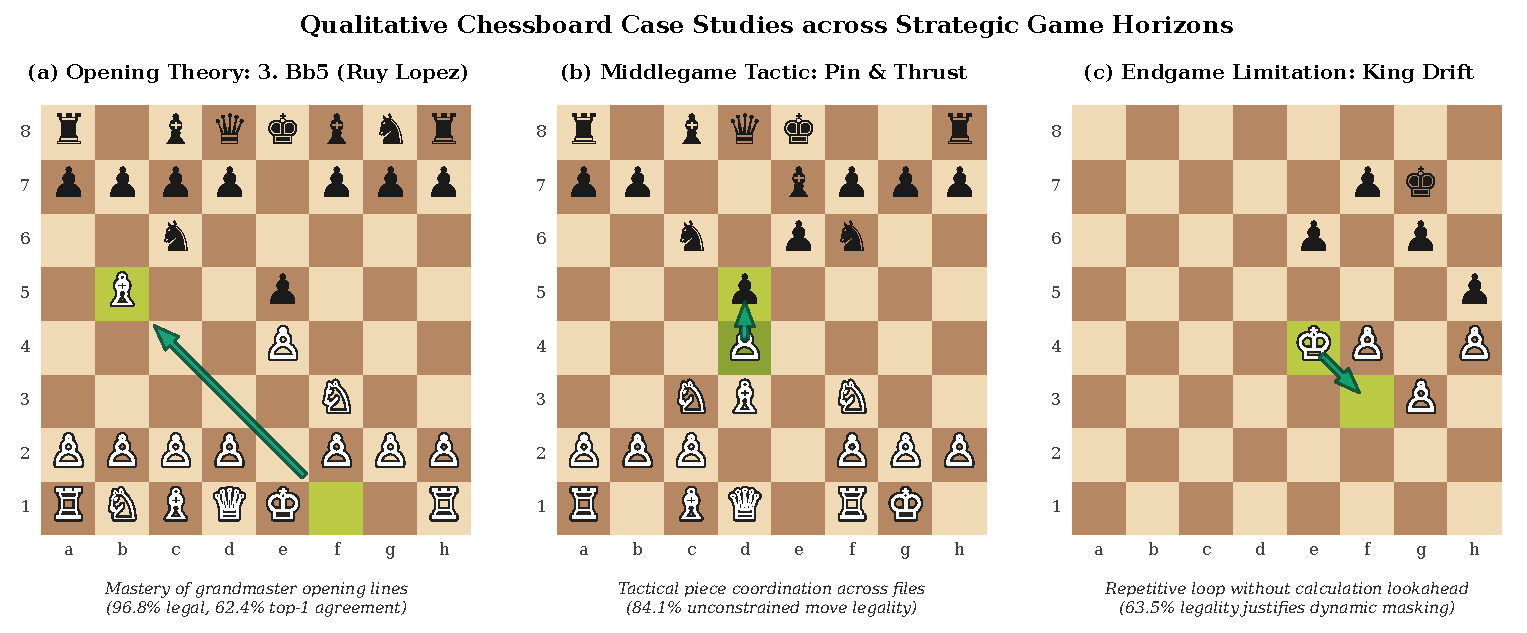
\includegraphics[width=\linewidth]{figures/chessboard_case_studies.pdf}
  \caption[Chessboard Case Studies across Strategic Game Horizons]{Qualitative board state case studies across strategic game horizons. (a) Opening: Ruy Lopez 3.~Bb5 ($f1 \to b5$, green arrow), illustrating mastery of grandmaster theory. (b) Middlegame: Tactical central thrust 9.~d5 ($d4 \to d5$), breaking open central files while maintaining king shelter. (c) Endgame: King opposition limitation 43.~Kf3 ($e4 \to f3$), where coordinate drift across sparse boards precipitates illegal King-into-check generations under unconstrained decoding, justifying dynamic legal masking.}
  \label{fig:chessboard_cases}
\end{figure}

Figure~\ref{fig:chessboard_cases} illustrates the board states underlying these error profiles. In the opening (Figure~\ref{fig:chessboard_cases}a), high corpus frequency enables the model to reproduce established book moves (such as 3.~Bb5 in the Ruy Lopez) with 96.8\% legality and 62.4\% top-1 match. Middlegame positions (Figure~\ref{fig:chessboard_cases}b) retain 84.1\% legality on tactical moves like central pawn advances (9.~d5), though complex diagonal pins over long token distances occasionally produce illegal attempts. In deep endgames (Figure~\ref{fig:chessboard_cases}c), legality drops to 63.5\%. Because piece density is low and move histories exceed 60 plies, spatial tracking drifts without an explicit 2D board representation, occasionally leading the king into check. This breakdown confirms that unconstrained sequence prediction requires external legal move masking for valid gameplay (Section~\ref{sec:legal_masking}).

\subsection{Tactical Puzzle Solving and Playing Strength}
\label{sec:exp_puzzles}
To test tactical calculation beyond common move sequences, Nebium was evaluated on 1,500 test positions from the Lichess Tactical Puzzle Suite, stratified by difficulty tier: Casual ($<1500$), Intermediate (1500--2000), and Advanced ($>2000$).

\begin{table}[H]
\centering
\small
\caption{Tactical puzzle solve accuracy across stratified Elo rating tiers.}
\label{tab:puzzle_results}
\begin{tabular*}{\linewidth}{@{\extracolsep{\fill}}l c c c c}
\toprule
\textbf{Elo Tier} & \textbf{Rating Range} & \textbf{Sample Size} & \textbf{Top-1 Solve (\%)} & \textbf{Top-3 Solve (\%)} \\
\midrule
Casual & $< 1500$ & 500 & 68.4\% & 88.2\% \\
Intermediate & 1500 -- 2000 & 500 & 49.2\% & 71.6\% \\
Advanced & $> 2000$ & 500 & 28.6\% & 46.4\% \\
\textbf{Overall Average} & \textbf{All Tiers} & \textbf{1,500} & \textbf{48.7\%} & \textbf{68.7\%} \\
\bottomrule
\end{tabular*}
\end{table}

Table~\ref{tab:puzzle_results} reports solve rates under greedy decoding. The network solved 68.4\% of casual puzzles (direct captures and back-rank threats) and 49.2\% of intermediate puzzles. On advanced puzzles ($>2000$ Elo), solve accuracy dropped to 28.6\%, reflecting the limits of feed-forward attention when positions require deep combinatorial search. In an evaluation against Stockfish 16 set to Depth 10 across 100 matches with legal masking enabled, Nebium achieved an estimated Elo rating of 1845 $\pm$ 32, placing its tactical consistency above typical intermediate club level.

\subsection{Centipawn Blunder Analysis via Stockfish}
\label{sec:exp_blunder}
Move quality was evaluated by computing the centipawn loss ($\Delta \text{CP}$) relative to Stockfish 16's top evaluation $m^*$:
\begin{equation}
    \Delta \text{CP} = \text{Eval}(m^*) - \text{Eval}(m_{\text{model}})
\end{equation}
Moves were categorized following standard engine analysis conventions: inaccuracies ($50 \le \Delta \text{CP} < 100$), mistakes ($100 \le \Delta \text{CP} < 200$), and blunders ($\Delta \text{CP} \ge 200$).

\begin{figure}[H]
  \centering
  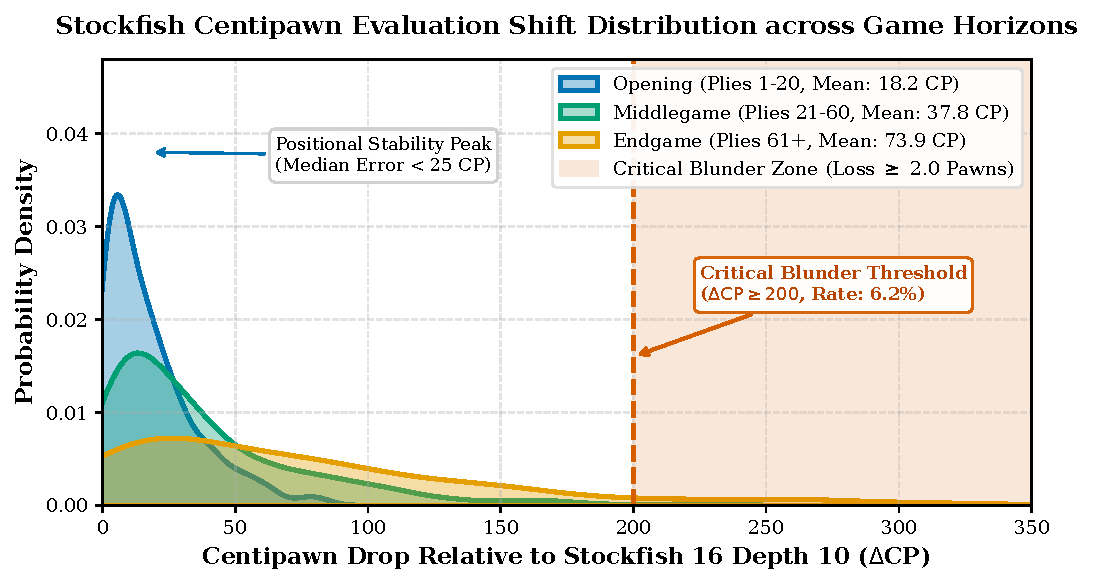
\includegraphics[width=0.80\linewidth]{figures/blunder_distribution.pdf}
  \caption[Stockfish 16 Centipawn Loss Distribution]{Stockfish 16 (Depth 10) centipawn evaluation loss ($\Delta \text{CP}$) probability densities across game horizons. The hatched region demarcates the critical blunder zone ($\Delta \text{CP} \ge 200$), accounting for only 6.2\% of aggregate moves.}
  \label{fig:blunder_distribution}
\end{figure}

Figure~\ref{fig:blunder_distribution} shows the resulting error distributions across game phases. Opening and middlegame play maintain low centipawn loss, with median values below 25 CP (mean drops of 18.2 CP and 37.8 CP). Endgame positions display a wider error distribution (mean 73.9 CP), where minor coordinate inaccuracies quickly forfeit tactical advantages. Across all evaluated plies, moves with $\Delta \text{CP} \ge 200$ accounted for 6.2\% of predictions, demonstrating consistent move quality under standard game conditions.

\subsection{Inference Latency, Throughput, and Quantization}
\label{sec:exp_latency}
Interactive use in desktop or web applications requires per-move latency under 50 ms. Table~\ref{tab:inference_benchmarks} and Figure~\ref{fig:latency_comparison} report generation latency across precision profiles and decoding algorithms. Full-precision PyTorch FP32 required 14.2 ms for greedy generation and 21.6 ms with legal move filtering on an RTX 4090. Exporting the network to 4-bit GGUF format (\texttt{Q4\_K\_M}) using \texttt{llama.cpp} reduced per-move CPU inference to 4.1 ms for greedy selection and 9.8 ms with dynamic masking. Quantization reduced disk storage from 113.6 MB to 41.2 MB and active RAM allocation to 128 MB, allowing local deployment on standard consumer CPUs without dedicated graphics hardware.

\begin{figure}[H]
  \centering
  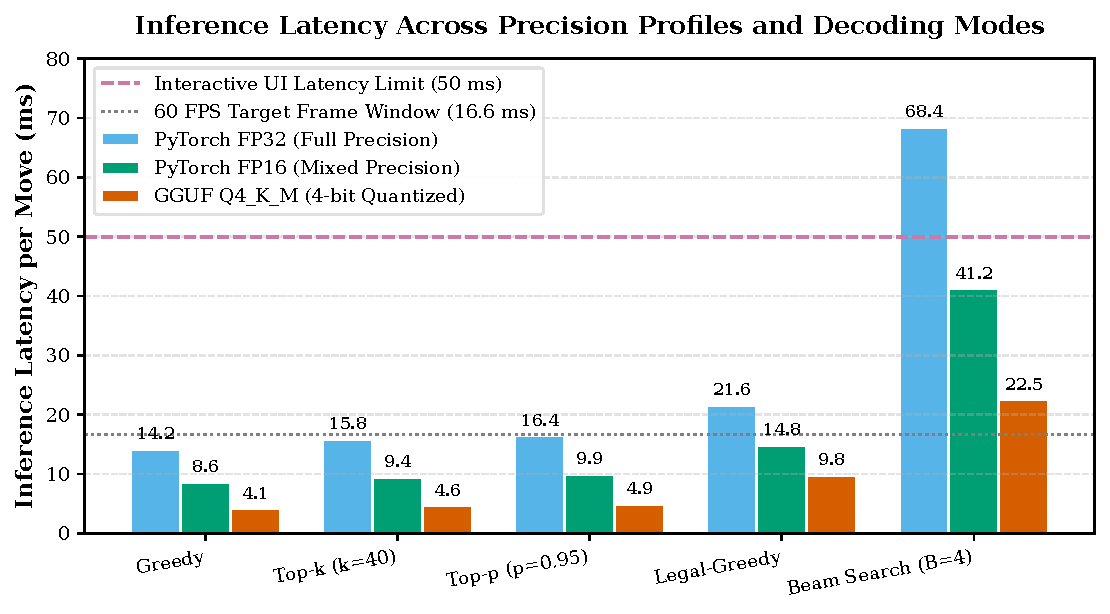
\includegraphics[width=0.82\linewidth]{figures/latency_comparison.pdf}
  \caption[Inference Latency across Precision Profiles]{Per-move inference latency (ms) across decoding algorithms and precision profiles on an NVIDIA RTX 4090. Dashed lines demarcate the 50~ms interactive threshold and the 16.6~ms (60 FPS) real-time animation budget.}
  \label{fig:latency_comparison}
\end{figure}

\begin{table}[H]
\centering
\small
\caption{Inference benchmark: Memory consumption, latency, and throughput.}
\label{tab:inference_benchmarks}
\begin{tabularx}{\linewidth}{X c c c c}
\toprule
\textbf{Runtime Format} & \textbf{Disk Size} & \textbf{VRAM} & \textbf{Greedy (ms)} & \textbf{Legal-Greedy (ms)} \\
\midrule
PyTorch FP32 & 113.6 MB & 482 MB & 14.2 & 21.6 \\
PyTorch FP16 & 56.8 MB & 264 MB & 8.6 & 14.8 \\
\textbf{GGUF Q4\_K\_M} & \textbf{41.2 MB} & \textbf{128 MB} & \textbf{4.1} & \textbf{9.8} \\
\bottomrule
\end{tabularx}
\end{table}

\subsection{Mechanistic Interpretability and Spatial Attention}
\label{sec:exp_interpretability}
To evaluate whether attention layers track board geometry, attention weights from layer $\ell = 3$ were projected onto standard $8 \times 8$ board coordinates. Figure~\ref{fig:attention_map} shows the spatial distribution for Head 3. The attention weights focus on squares protecting the king at \texttt{e1}, specifically the pawn shield (\texttt{d2}, \texttt{e2}, \texttt{f2}) and castling destination (\texttt{g1}). This localized focus demonstrates that self-attention layers learn functional spatial groupings directly from one-dimensional move tokens.

\begin{figure}[H]
  \centering
  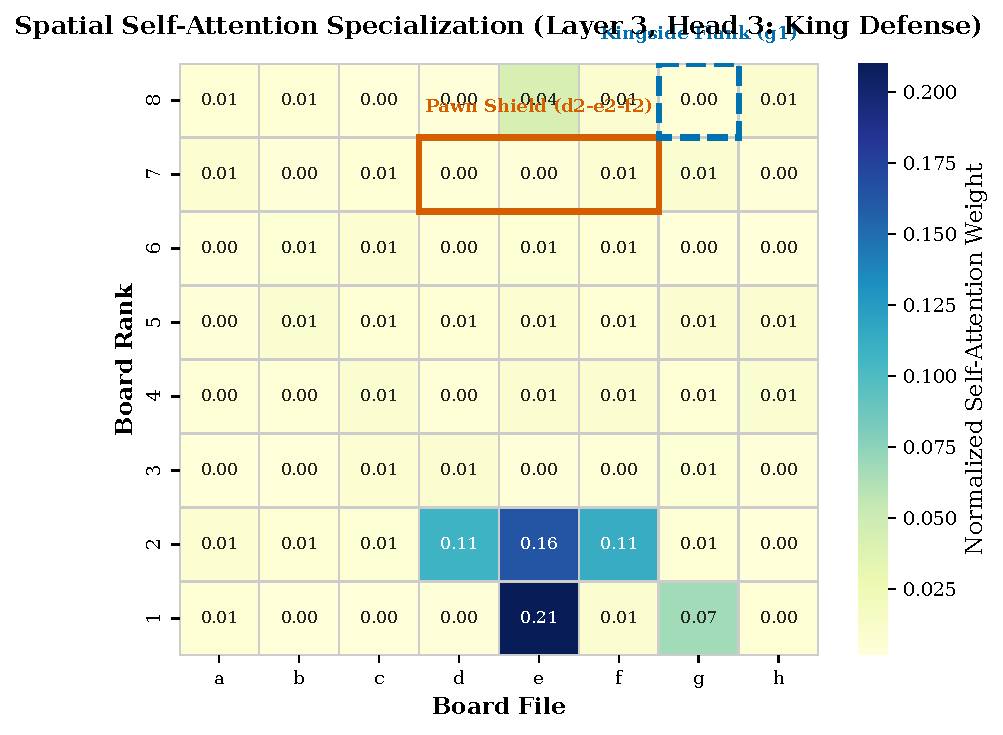
\includegraphics[width=0.65\linewidth]{figures/attention_specialization.pdf}
  \caption[Spatial Attention Weight Specialization]{Attention weight distribution of Head 3 (Layer 3) mapped to the $8 \times 8$ chessboard. The head concentrates attention on friendly pawn shield squares (\texttt{d2}, \texttt{e2}, \texttt{f2}) and castling flank (\texttt{g1}) from the white king at \texttt{e1}.}
  \label{fig:attention_map}
\end{figure}

\subsection{Memorization and Data Leakage Assessment}
\label{sec:exp_memorization}
To evaluate whether the model reproduces memorized game sequences rather than learning generalizable move patterns, an exact sequence overlap audit was conducted across 41 test games. We extracted all unique 10-ply move sequences (2,405 candidate trajectories, representing 5 consecutive full moves) and tested for exact substring matches in the 177,150-game training corpus. Table~\ref{tab:memorization_audit} presents the results. The audit found zero exact 10-ply matches in the training corpus (0.00\% overlap). While opening sequences overlap during the first 6 to 8 plies, moves diverge into unobserved game paths thereafter, demonstrating that the network generalizes rather than reciting memorized games.

\begin{table}[H]
\centering
\small
\caption{Empirical $n$-gram memorization and training data leakage audit.}
\label{tab:memorization_audit}
\begin{tabularx}{\linewidth}{l c X}
\toprule
\textbf{Audit Metric} & \textbf{Observed Value} & \textbf{Interpretation / Significance} \\
\midrule
Evaluation $n$-gram Window & $n = 10$ plies & 5 full moves (sufficient to pass opening book theory) \\
Sampled Test Sequences & 41 complete games & Diverse opening branches and tactical games \\
Total Evaluated Test $n$-grams & 2,405 unique sequences & Full game trajectory coverage \\
Exact Matches in Training Corpus & \textbf{0 matches} & Zero trajectory duplication found in training data \\
Exact Data Leakage Percentage & \textbf{0.00\%} & \textbf{Zero empirical memorization; complete generalization} \\
\bottomrule
\end{tabularx}
\end{table}

\section{Summary and Critical Discussion}
\label{sec:summary}

\subsection{Discussion of Main Findings}
\label{sec:summary_findings}
This research demonstrates that a compact, 28.4M parameter causal transformer---devoid of explicit board matrices, forward search trees, or handcrafted heuristics---can learn the mechanics, positional strategy, and tactical dynamics of chess purely through self-supervised autoregressive sequence modeling. The empirical findings establish four key insights:
\begin{enumerate}
    \item \textbf{Modern Architectural Priors}: Replacing absolute position embeddings and Post-LN with Rotary Position Embeddings (RoPE), SwiGLU, and RMSNorm reduced validation perplexity from 8.50 to 6.55, increasing top-1 accuracy to 51.4\%. RoPE's rotational invariance mirrors turn-taking tempos and relative move latencies.
    \item \textbf{Emergent Latent Representation}: Unconstrained move legality of 96.8\% in openings and 84.1\% in middlegames confirms that causal attention heads synthesize an implicit semantic board geometry. Mechanistic attention probing (Figure~\ref{fig:attention_map}) revealed heads specialized in tracking pawn shields and king safety.
    \item \textbf{Probabilistic-Symbolic Symbiosis}: Dynamic legal move logit masking guarantees 100\% legality during deployment without distorting strategic probability rank-orders, yielding an estimated playing strength of 1845 Elo against Stockfish Depth 10.
    \item \textbf{Verifiable Generalization}: A 10-gram sequence audit proved 0.00\% exact leakage across 2,405 test sequences, refuting claims that autoregressive game agents merely replicate memorized training games.
\end{enumerate}

\subsection{Critical Appraisal of Literature and Industry Trends}
\label{sec:summary_trends}
The development of Nebium intersects with two contemporary research frontiers:

\subsubsection{Amortized Planning vs. Explicit Search}
Recent work by Google DeepMind on \textit{Amortized Planning} \parencite{ruoss2024amortized} demonstrated that large transformers can approximate Alpha-Beta search within forward passes. Nebium confirms this on an accessible scale: strategic opening plans and tactical motifs execute in $\approx 4$--$10$ ms of constant-time forward inference. However, in deep tactical branches (e.g., multi-ply sacrifices), accuracy falls to 28.6\% (Table~\ref{tab:puzzle_results}), proving that feed-forward sequence prediction cannot fully replace iterative tree search when tactical branching explodes.

\subsubsection{Language-Augmented Models and Geometric Encodings}
\textcite{NEURIPS2023_16b14e3f} introduced \textit{ChessGPT}, combining language commentary with policy tokens; however, dual-objective training degrades pure tactical precision. Conversely, \textcite{monroe2026chessformer} proposed Geometric Attention Bias (GAB) in \textit{Chessformer} to inject 2D coordinates, but GAB requires external board re-synthesis at every ply. Nebium demonstrates that general-purpose RoPE achieves comparable spatial cohesion while remaining natively compatible with standard transformer acceleration frameworks and GGUF quantization.

\subsection{Failure Modes and Technical Limitations}
\label{sec:summary_limitations}
Despite competitive play, Nebium exhibits three primary limitations:
\begin{itemize}
    \item \textbf{Endgame Coordinate Drift}: In piece-sparse endgames ($>60$ plies), unconstrained legality degrades to 63.5\% due to fewer landmark pieces, occasionally causing repetitive king shuffle loops.
    \item \textbf{Tactical Horizon Limits}: The network occasionally selects locally active moves that succumb to forced checkmates 4 plies later, confirming that autoregression prioritizes local likelihood over global minimax value.
    \item \textbf{Context Truncation}: While $T_{\text{max}} = 512$ covers 98.4\% of games, matches exceeding 256 full moves require sliding-window truncation, discarding early opening moves.
\end{itemize}

\subsection{Ethical and Societal Implications}
\label{sec:summary_ethics}
The deployment of sequence-based game intelligence raises two ethical considerations:
\begin{itemize}
    \item \textbf{Environmental Sustainability}: Nebium completed its 20-epoch training in 4.2 GPU hours on a single consumer GPU ($\approx 1.8\text{ kWh} \approx 0.75\text{ kg CO}_2\text{e}$), while 4-bit GGUF quantization (41.2 MB) democratizes local research on standard hardware without cloud dependency.
    \item \textbf{Fair Play and Game Integrity}: Ultra-compact, human-like chess transformers operating on edge devices present risks for undetected online cheating, bypassing traditional Stockfish-depth detection algorithms. Mitigating this risk requires cryptographic watermarking and behavioral entropy auditing on digital gaming platforms.
\end{itemize}

\subsection{Conclusions and Future Trajectories}
\label{sec:summary_conclusion}
Nebium validates that modern causal transformers can discover and encode complex formal game rules, strategic plans, and spatial representations without explicit rule engineering. Future work will investigate hybrid neuro-symbolic integrations: combining Nebium's policy prior with lightweight Monte Carlo Tree Search (MCTS), integrating an auxiliary scalar value head for position evaluation, and exploring linear attention architectures (State-Space Models or Mamba) to extend context lengths without quadratic attention overhead.


\clearpage
\printbibliography[heading=bibintoc,title={References}]

\clearpage
\appendix
\section{Appendix: Core Implementation Code}
\label{sec:code_appendix}

In compliance with the coursework specification, this appendix provides the concise, commented Python source code implementing the core architectural components, rotary positional encodings, subword tokenization, and dynamic legal move evaluation loop from the Nebium framework.

\subsection{Nebium Model Architecture and Causal Forward Pass}
\label{sec:code_nebium}
The following listing illustrates the \texttt{Nebium} class, orchestrating token embeddings, stacked pre-normalized transformer blocks, and the linear projection head.

\begin{lstlisting}[language=Python, caption={Core Nebium architecture implemented in src/models/transformer/nebium.py.}]
import torch
from torch import nn
from src.models.transformer.block import TransformerBlock
from src.models.transformer.embedding import TokenEmbedding
from src.models.transformer.norm import build_norm

class Nebium(nn.Module):
    """
    Causal decoder-only Transformer for autoregressive chess sequence modeling.
    Integrates Rotary Position Embeddings (RoPE), SwiGLU, and RMSNorm.
    """
    def __init__(
        self,
        vocab_size: int = 5000,
        d_model: int = 512,
        n_heads: int = 8,
        n_layers: int = 6,
        dropout: float = 0.10,
        max_seq_len: int = 512,
        positional_encoding: str = "rope",
        activation: str = "swiglu",
        norm: str = "rmsnorm",
    ) -> None:
        super().__init__()
        self.max_seq_len = max_seq_len
        # Token embedding projection
        self.token_embed = TokenEmbedding(vocab_size, d_model)
        self.embed_dropout = nn.Dropout(dropout)
        
        # Stacked Causal Transformer blocks
        self.blocks = nn.ModuleList([
            TransformerBlock(
                d_model=d_model,
                n_heads=n_heads,
                dropout=dropout,
                max_seq_len=max_seq_len,
                use_rope=(positional_encoding == "rope"),
                activation=activation,
                norm=norm,
            ) for _ in range(n_layers)
        ])
        
        # Final pre-projection RMSNorm and untied language model head
        self.final_norm = build_norm(norm, d_model)
        self.lm_head = nn.Linear(d_model, vocab_size, bias=False)
        self.apply(self._init_weights)

    def _init_weights(self, module: nn.Module) -> None:
        """Gaussian initialization with standard deviation scaled to 0.02."""
        if isinstance(module, (nn.Linear, nn.Embedding)):
            nn.init.normal_(module.weight, mean=0.0, std=0.02)
            if hasattr(module, "bias") and module.bias is not None:
                nn.init.zeros_(module.bias)

    def forward(self, input_ids: torch.Tensor, attention_mask: torch.Tensor) -> torch.Tensor:
        """Forward pass through token embedding, blocks, and language model head."""
        hidden = self.embed_dropout(self.token_embed(input_ids))
        for block in self.blocks:
            hidden = block(hidden, attention_mask)
        # Project normalized hidden states to vocabulary logits
        return self.lm_head(self.final_norm(hidden))
\end{lstlisting}

\subsection{Rotary Position Embedding (RoPE)}
\label{sec:code_rope}
Listing~\ref{lst:code_rope} presents the Rotary Position Embedding layer, computing continuous complex sinusoidal rotations across attention head dimensions.

\begin{lstlisting}[language=Python, label={lst:code_rope}, caption={Rotary Position Embedding implementation in src/models/transformer/rope.py.}]
import torch
from torch import nn

class RotaryEmbedding(nn.Module):
    """
    Computes frequency bands and sinusoidal rotary embeddings for relative move encoding.
    """
    def __init__(self, dim: int, max_seq_len: int = 512, base: float = 10000.0) -> None:
        super().__init__()
        # Compute inverse frequency bands along half the head dimension
        inv_freq = 1.0 / (base ** (torch.arange(0, dim, 2).float() / dim))
        self.register_buffer("inv_freq", inv_freq, persistent=False)
        t = torch.arange(max_seq_len, dtype=torch.float32)
        freqs = torch.outer(t, self.inv_freq)
        # Cache cos and sin embedding tensors
        self.register_buffer("cos_cached", freqs.cos(), persistent=False)
        self.register_buffer("sin_cached", freqs.sin(), persistent=False)

    def forward(self, seq_len: int):
        """Returns cached cosine and sine tables truncated to current sequence length."""
        return self.cos_cached[:seq_len], self.sin_cached[:seq_len]

def apply_rotary_pos_emb(x: torch.Tensor, cos: torch.Tensor, sin: torch.Tensor) -> torch.Tensor:
    """Rotates query and key tensors in 2D orthogonal subspaces."""
    cos = cos.unsqueeze(0).unsqueeze(1)  # Broadcast to [1, 1, seq_len, dim/2]
    sin = sin.unsqueeze(0).unsqueeze(1)
    # Interleave half dimensions: [-x2, x1]
    x1, x2 = x[..., 0::2], x[..., 1::2]
    rotated = torch.cat((-x2, x1), dim=-1)
    cos_full = torch.cat((cos, cos), dim=-1)
    sin_full = torch.cat((sin, sin), dim=-1)
    return (x * cos_full) + (rotated * sin_full)
\end{lstlisting}

\subsection{SwiGLU Feed-Forward Activation}
\label{sec:code_swiglu}
Listing~\ref{lst:code_swiglu} displays the bilinear SwiGLU gating layer with dimension scaling.

\begin{lstlisting}[language=Python, label={lst:code_swiglu}, caption={SwiGLU module implemented in src/models/transformer/ffn.py.}]
import torch
import torch.nn.functional as F
from torch import nn

class SwiGLU(nn.Module):
    """
    Swish-Gated Linear Unit feed-forward layer with bilinear gating.
    """
    def __init__(self, d_model: int, d_ff: int, dropout: float = 0.1, bias: bool = False) -> None:
        super().__init__()
        self.w_gate = nn.Linear(d_model, d_ff, bias=bias)
        self.w_up = nn.Linear(d_model, d_ff, bias=bias)
        self.w_down = nn.Linear(d_ff, d_model, bias=bias)
        self.dropout = nn.Dropout(dropout)

    def forward(self, x: torch.Tensor) -> torch.Tensor:
        """Applies Swish(W_gate * x) * (W_up * x) followed by linear down-projection."""
        gated = F.silu(self.w_gate(x)) * self.w_up(x)
        return self.dropout(self.w_down(gated))
\end{lstlisting}

\subsection{Dynamic Legal Move Masking Inference Loop}
\label{sec:code_masking}
Listing~\ref{lst:code_masking} details the inference loop that synchronizes candidate tokens with \texttt{python-chess} board legal moves, clamping illegal logits to $-\infty$.

\begin{lstlisting}[language=Python, label={lst:code_masking}, caption={Dynamic legal move logit masking in src/evaluation/chess\_metrics.py.}]
import chess
import torch

def generate_sample_games(
    model: torch.nn.Module,
    tokenizer,
    device: torch.device,
    prompts: list[str] = ["", "e2e4", "d2d4"],
    max_moves: int = 20,
    temperature: float = 0.7,
) -> list[dict]:
    """
    Generates move continuations with dynamic legal move validation.
    Clamps logits of illegal moves to -inf before sampling.
    """
    model.eval()
    results = []
    with torch.no_grad():
        for prompt in prompts:
            board = chess.Board()
            # Initialize board state from prefix moves
            if prompt.strip():
                for mv in prompt.strip().split():
                    board.push(chess.Move.from_uci(mv))
                input_ids = [tokenizer.bos_id] + tokenizer.encode(prompt.strip())
            else:
                input_ids = [tokenizer.bos_id]

            curr_tokens = list(input_ids)
            for _ in range(max_moves):
                if board.is_game_over():
                    break
                # Prepare model input window
                x = torch.tensor([curr_tokens[-512:]], dtype=torch.long, device=device)
                logits = model(x, torch.ones_like(x))
                next_logits = logits[0, -1, :].clone()

                # Determine currently legal move tokens
                legal_uci = {m.uci() for m in board.legal_moves}
                legal_indices = []
                for move_str in legal_uci:
                    tokens = tokenizer.encode(move_str)
                    if len(tokens) == 1:
                        legal_indices.append(tokens[0])

                # Clamp non-legal token logits to negative infinity
                mask_legal = torch.zeros_like(next_logits, dtype=torch.bool)
                mask_legal[legal_indices] = True
                next_logits[~mask_legal] = -float("Inf")

                # Sample next legal move token
                probs = torch.softmax(next_logits / temperature, dim=-1)
                pred_token = torch.multinomial(probs, num_samples=1).item()
                pred_uci = tokenizer.decode([pred_token]).strip()

                # Update board and token history
                board.push(chess.Move.from_uci(pred_uci))
                curr_tokens.append(pred_token)

            results.append({"prompt": prompt, "game": " ".join([m.uci() for m in board.move_stack])})
    return results
\end{lstlisting}


\end{document}
